\documentclass[report/main.tex]{subfiles}

% A description and illustration of the:

% - Design of your ITU-MiniTwit systems
% - Architecture of your ITU-MiniTwit systems
% - All dependencies of your ITU-MiniTwit systems on all levels of abstraction and development stages.
    % - That is, list and briefly describe all technologies and tools you applied and depend on.
% - Important interactions of subsystems
% - Describe the current state of your systems, for example using results of static analysis and quality - assessment systems.
% - Finally, describe briefly, if the license that you have chosen for your project is actually compatible with - the licenses of all your direct dependencies.

% Double check that for all the weekly tasks (those listed in the schedule) you include the corresponding information.

\begin{document}
    \section{System's Perspective}
    \label{Sec:systems_perspective}
    
        \subsection{Architecture of the system}
        \label{subsec:architecture_of_system}
        % https://stackoverflow.com/questions/704855/software-design-vs-software-architecture
        % https://codeburst.io/software-architecture-the-difference-between-architecture-and-design-7936abdd5830
        % https://softwareengineering.stackexchange.com/questions/361371/what-is-a-proper-diagram-to-describe-software-architecture#:~:text=In%20UML%20there%20is%20no%20single%20architecture%20diagram%20that%20summarizes%20everything.&text=For%20the%20layers%2C%20the%20logical,also%20components%2C%20and%20use%20cases.
            
            % \begin{wrapfigure}{r}{0.4\textwidth}
            %     \centering
            %     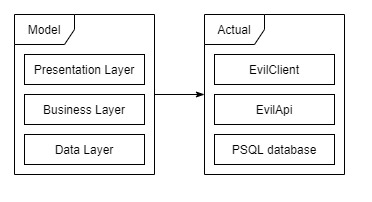
\includegraphics[width=0.4\textwidth]{report/images/EvilTwitter-Three Layered Architecture.jpg}
            %     \caption{TODO}
            %     \label{fig:three-layered-architecture}
            % \end{wrapfigure}
            
            % TODO: too much arguing?!?!
            This section will start with a walk through of the overall structure of the project, followed by a further explanation of its sub-parts.
            
            The general structure of the project is a Three Layered Architecture, because it formed a nice separation of concerns in the application. This resulted in three applications namely, EvilClient for the presentation tier, EvilApi for the business/logic tier and the PostgreSQL (PSQL) database cluster for the data tier. For an overview of the architecture, see the model diagram in figure \ref{fig:model-diagram}.
            
            \begin{figure}[H]
                \centering
                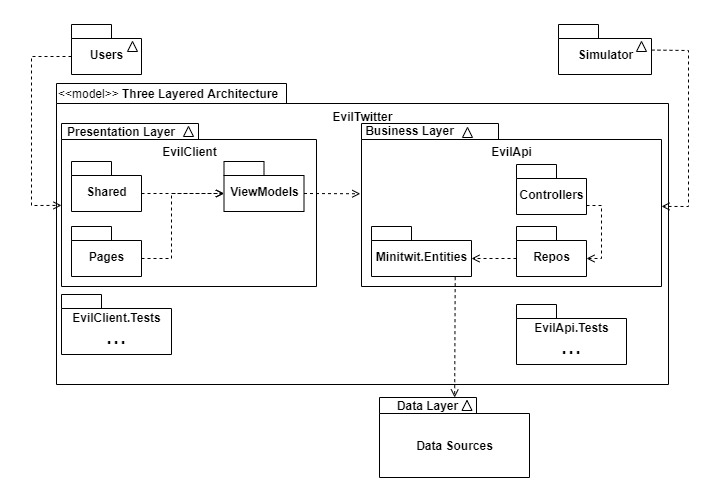
\includegraphics[width=0.8\textwidth]{report/images/EvilTwitter-Model Diagram - Evil Corp.jpg}
                \caption{Model diagram of the project, depicting important folders of the source code. Arrows have been added to show the flow of data in the system which also coincides with dependencies between parts of the applications. The flow of data starts at the user or simulator and pointing to the next source file that would further the request along, resulting in all arrows leading to the database at the bottom}
                \label{fig:model-diagram}
            \end{figure}
            
            By following the Three Layered Architecture only two paths of communication exists, where both use a different architecture. First path is between EvilClient and EvilApi, the second path is between EvilApi and the database. This flow can be seen in figure \ref{fig:model-diagram} and \ref{fig:deployment-diagram}.
            
            \begin{figure}
                \centering
                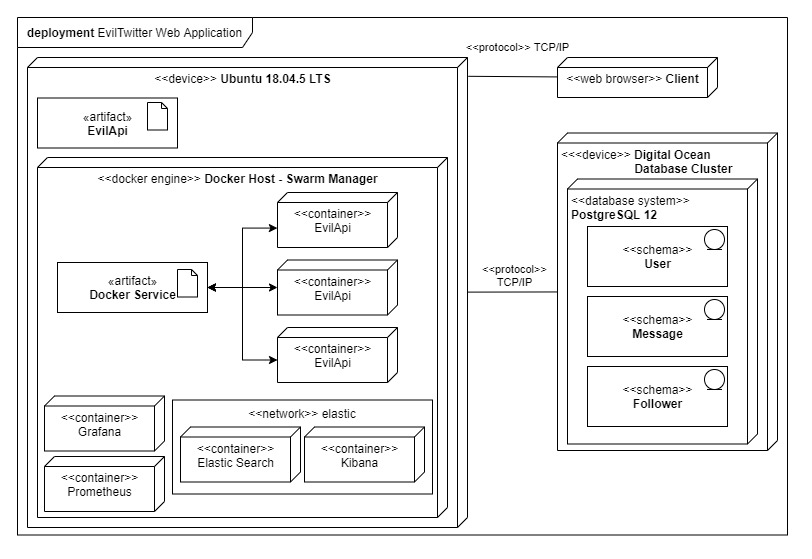
\includegraphics[width=0.8\textwidth]{report/images/EvilTwitter-Deployment Diagram - Evil Corp.jpg}
                \caption{Deployment diagram of the project EvilTwitter showing the current state of the project}
                \label{fig:deployment-diagram}
            \end{figure}
            
            Communication between EvilClient and EvilApi is done via TCP/IP using the http protocol to deliver optional JSON files in the http request. The EvilApi follows the REST Architecture (Representational State Transfer), while the EvilApi and the database communicates via an ORM (Object Relational Mapping) specifically the EF Core framework.
            
            Finally, as seen in figure \ref{fig:deployment-diagram} the application attempts to create a microservice by orchestrating some of the docker containers in a swarm mode, to utilise load balancing and making the service more resilient. This had some shortcomings by having only the EvilApi as a microservice and by the EvilClient and EvilApi talking together over the droplet's ports instead of internally i.e. the docker network.
    
        \subsection{Design of the system}
        \label{subsec:design_of_system}
        % https://stackoverflow.com/questions/704855/software-design-vs-software-architecture
        % https://codeburst.io/software-architecture-the-difference-between-architecture-and-design-7936abdd5830 
        % https://softwareengineering.stackexchange.com/questions/361371/what-is-a-proper-diagram-to-describe-software-architecture#:~:text=In%20UML%20there%20is%20no%20single%20architecture%20diagram%20that%20summarizes%20everything.&text=For%20the%20layers%2C%20the%20logical,also%20components%2C%20and%20use%20cases.
            The architecture outlined in section \ref{subsec:architecture_of_system} separated the application into 3 distinct entities. Their design will be covered separately in the following sections.
            
            \subsubsection{Design of EvilClient}
            \label{subsubsec:architexture_of_evilclient}
                The main responsibility of the EvilClient is to display data from the database to the user sent by the EvilApi, and handle inputs from the user that could manipulate data in the database. Hence, the responsibility of the EvilClient is data conversion between displaying data to the user and converting user input to usable data in the database. Thereby, the MVVM (Model-View-View-Model) pattern was chosen (\cite{ms-mvvm}).
                
                Of notice should be the Pages, Shared, ViewModels folders of the EvilClient folder. Here Pages and Shared contains the View part of MVVM. To display the razor files in a browser the Microsoft Blazor Framework\footnote{\href{https://dotnet.microsoft.com/apps/aspnet/web-apps/blazor}{Blazor framework}} converts the code into a application that is executable in a web browser. The ViewModels folder holds the code that converts data from the EvilApi into usuable information to the user, and vice versa converts input from the client into data that is usable for the EvilApi.
    
            \subsubsection{Design of EvilApi}
            \label{subsubsec:architecture-of-evilApi}
                EvilApi is a REST \cite{rest} Api that updates a database according to the requests sent. To handle the conversion from C\# data types to PostreSQL data types the application is using an ORM, which in this case is the EF Core framework\footnote{\href{https://docs.microsoft.com/en-us/ef/core/}{EF core framework}}.
            
            \subsubsection{Design of the database}
            \label{subsubsec:design-of-the-database}
                As seen on figure \ref{fig:deployment-diagram} the data consisted of three different types and was very structured, hence a relational database seemed like an optimal choice. From the many SQL flavours, we decided to use Postgres, due to its open source nature. The database was arranged in a cluster structure to increase scalability, data redundancy and availability.
        
        \subsection{Dependencies}
        \label{subsec:dependencies}
            Below is a summarised version of the dependency graph on Github, where all the dependencies of the project is listed under the component depending on it.\footnote{\href{https://github.com/gustavjohansen98/E-vil-Corp/network/dependencies}{Dependency graph}}. Important dependencies will be elaborated on later, in sections where they are deemed relevant.
        
            \begin{table}[H]
                \small
                \begin{tabular}{|p{4.5cm}|p{4.5cm}|p{2.5cm}|p{3cm}|}
                    \hline
                    apache 2                            & MIT                           & BSD 3clause & PostgresQL license \\ \hline
                    AspNetCore.Diagnostics.\newline HealthChecks & Newtonsoft.Json               & moq4        & npgsql/efcore.pg   \\
                    code-cracker                        & ProfanityDetector             &             &                    \\
                    dotnet/efcore                       & prometheus-net                &             &                    \\
                    aspnet/Diagnostics                  & prometheus-net.SystemMetrics  &             &                    \\
                    serilog-aspnetcore                  & RehanSaeed/Serilog.\newline Exceptions &             &                    \\
                    serilog-enrichers-environment       & Swashbuckle.AspNetCore        &             &                    \\
                    serilog-sinks-debug                 & coverlet                      &             &                    \\
                    serilog-sinks-elasticsearch         & vstest                        &             &                    \\
                    Roslynator                          &                               &             &                    \\
                    xunit                               &                               &             &                    \\
                    visualstudio.xunit                  &                               &             &                    \\ \hline
                \end{tabular}
                \caption {All the dependencies EvilClient and EvilApi is using grouped by license} 
                \label{tab:title}
            \end{table}
            
            %A dependency graph for all used dependencies can be found in our GitHub repository\footnote{\hyperlink{Dependeny graph}{https://github.com/gustavjohansen98/E-vil-Corp/network/dependencies}}. %TODO: could be a part of the table text
    
        \subsection{Interactions of subsystems}
            Taking the current state of the system as a starting point with only one droplet, helps describe the interactions of the subsystems. Hence, a setup having multiple droplets is possible and each droplet would be identical in regard to interactions of subsystems. The setup is depicted in figure \ref{fig:component-diagram}, following the Three Layered Architecture presented in section \ref{subsec:architecture_of_system}, in this example the presentation tier and business tier is located on the same droplet, the data tier located on another device. Also, it is observed that the EvilClient communicates directly with the EvilApi\footnote{Note should be taken that the EvilClient actually sends out an http request that leaves the droplet, only to return shortly after. This is not optimal and the services should talk internally on the droplet i.e. via the docker network}. Via sending http requests back and forth, as described in section \ref{subsec:architecture_of_system}. Furthermore, the simulator talks directly to the EvilApi in the same manner as the EvilClient, which leaves only the EvilApi communicating directly with the database.
    
            \begin{figure}[H]
                \centering
                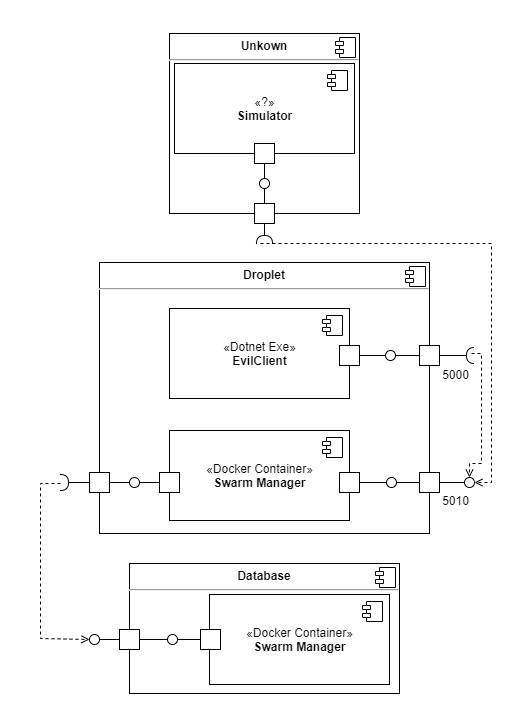
\includegraphics[width=0.8\textwidth]{report/images/EvilTwitter-Component Diagram - Evil Corp.jpg}
                \caption{Component diagram depicting the interactions of the subsystems that make up the EvilTwitter project}
                \label{fig:component-diagram}
            \end{figure}
            
        \subsection{Current state of the systems}
        \label{subsec:current-state-of-the-system}
            To assess the state of the system, we'll have a look and discussion of the SonarCloud report produced in the CI pipeline from the main branch.\footnote{\href{https://sonarcloud.io/dashboard?id=gustavjohansen98_E-vil-Corp}{SonarCloud report}}
            
            \begin{figure}[H]
                \centering
                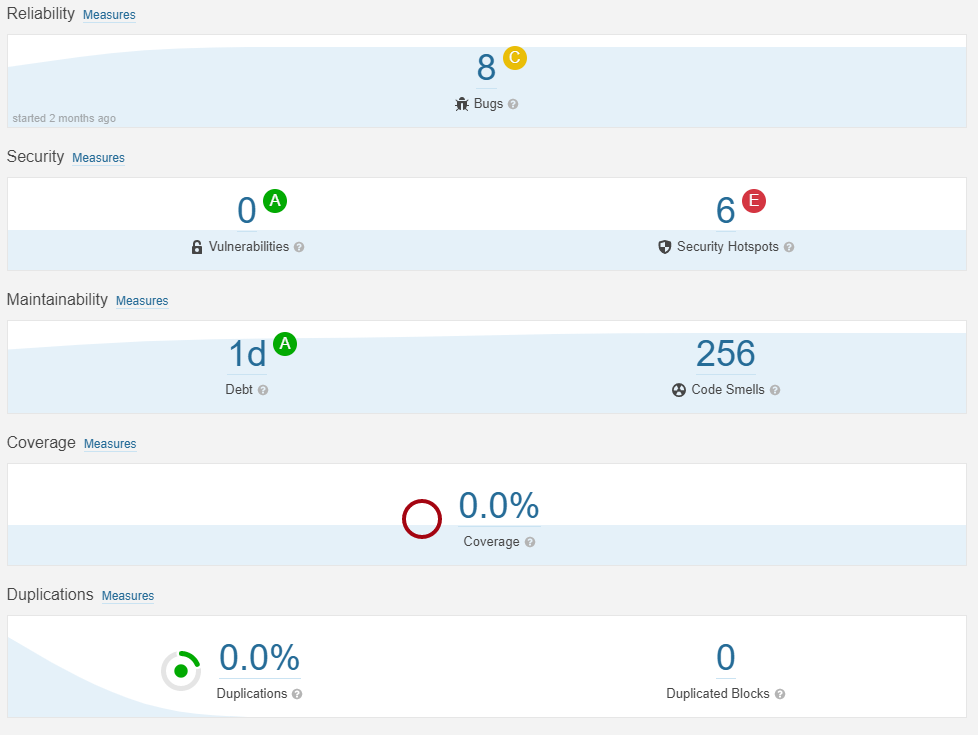
\includegraphics[width=0.7\textwidth]{report/images/SonarCloud Report.png}
                \caption{SonarCloud report of the EvilApi. Note that there's a mistake in the latter reports as it couldn't find the tests written for the application}
                \label{fig:sonarcloud}
            \end{figure}
            
            By looking at the security hotspots 3 clear risks can be seen:
            
            \begin{itemize}
                \item Use of MD5 hasher
                \item Logging Injection
                \item Use of the http protocol
            \end{itemize}
            
            From this the MD5 hash was kept due to the lack of a password reset function, as the application was first deployed with a MD5 hash, hence users made initially would not be able to log in. Though, the MD5 hash is used in the creation of the user avatar, this only hashes the email, and since this is publicly available on people's profiles, it is not seen as a risk.
            
            % TODO: Fix this, moving the logs shouldn't make us less worried
            Due to messages received only containing hashed information, logging injection is seen as less of a risk. Furthermore, the application is in a process of moving the logs to a separate database, hence a solution might become invalid and have to be redone shortly after implementation.

            It is of course not recommended to make use of the http protocol instead of the https protocol, but we simply didn't prioritise getting a https certificate\footnote{\href{https://docs.microsoft.com/en-us/aspnet/core/security/enforcing-ssl?view=aspnetcore-5.0\&tabs=visual-studio}{https certificate for ASP.NET core}} for the ASP.NET core framework used.
            
            We have an overall acceptable technical debt of 8 hours\footnote{\href{https://docs.sonarqube.org/latest/user-guide/metric-definitions/\#header-4}{SonarCloud documentation}} with 256 code smells to cover.
    
        \subsection{Software license agreement}
            As listed in section \ref{subsec:dependencies}, we have 21 direct dependencies. 11 of them are licensed under Apache version 2\footnote{\href{https://www.apache.org/licenses/LICENSE-2.0}{apache}}, 8 of them under the MIT license\footnote{\href{https://opensource.org/licenses/MIT}{MIT license}}, while the BSD 3-clause\footnote{\href{https://opensource.org/licenses/BSD-3-Clause}{opensource.org}} and PostgresQL license\footnote{\href{https://www.postgresql.org/about/licence/}{psql}} cover 1-1 dependency each. Since all these licences are permissive, we had a lot of freedom to choose how to license our software. While we must preserve the original license notices in the files which use code covered by the aforementioned licences, we are permitted to license the project \textit{as a whole} as we see fit. Therefore, to make sure third parties don't profit from our work, we released the project under the GPL version 3\footnote{\href{https://www.gnu.org/licenses/gpl-3.0.en.html}{gnu}}.
    
\end{document}